\documentclass[
	12pt,
    a4paper,
    egregdoesnotlikesansseriftitles, % Überschriften haben gleichen Font wie restlicher Text
    toc=chapterentrywithdots,
    oneside, openany,
    % twoside,openright,
    titlepage,
    parskip=half,
    headings=normal,  % reduces heading size
    listof=totoc,
    bibliography=totocnumbered,
    index=totoc,
    captions=tableheading,  % caption below table
    % chapterprefix,
    listof=flat,
    numbers=noenddot, % kein Punkt nach Nummerierung im Inhaltsverzeichnis
    final]
    {scrbook}
    
% details about your thesis
\newcommand{\titel}{Discrimination in Algorithms (Face Recognition)}
\newcommand{\artderarbeit}{Studienarbeit}  % {Bachelorarbeit,Masterarbeit}
\newcommand{\autor}{Ronny Pollak}
\newcommand{\modul}{Intercultural Communications} 
%\newcommand{\modulzusatz}{Strategien,\,Architekturen\,und\,Algorithmen}
\newcommand{\matrikelnr}{3694422}
\newcommand{\dozent}{Wolfgang Jockusch}
\newcommand{\abgabedatum}{27.01.2023}
\newcommand{\keywords}{key, words}
%\newcommand{\studentname}{key, words}
%\newcommand{\studentMatnr}{key, words}
\newcommand{\studentStudiengang}{Master Informatik}


% custom head and foot
\usepackage[automark]{scrlayer-scrpage}
\pagestyle{scrheadings}
\ihead{\headmark}
\chead{}
\ohead{\pagemark}
\renewcommand*\chaptermarkformat{\chapappifchapterprefix{\ }% 
  \thechapter.\enskip}
% anderenfalls zu viel Abstand von Titeln zu oberem Seitenrand
\RedeclareSectionCommand[afterindent=false,beforeskip=0pt]{chapter}

\RedeclareSectionCommand[tocindent=0pt]{section}
\RedeclareSectionCommand[tocindent=0pt]{subsection}
%\RedeclareSectionCommand[tocnumwidth=70pt]{chapter}

\usepackage{scrhack}

% other packages
\usepackage[utf8]{inputenc}
\usepackage[T1]{fontenc}
\usepackage{lmodern,relsize,textcomp,csquotes}
\usepackage{amsmath,amsfonts}
\usepackage[ngerman,english]{babel}  % flip for German thesis
\usepackage[final]{graphicx}
\usepackage{setspace,geometry,xcolor}
\usepackage{makeidx}
\usepackage{paralist,ifthen,todonotes}
\usepackage{url}
\usepackage[toc]{glossaries}
\usepackage{pdfpages}

% table setup
\usepackage{longtable}
\usepackage{array}
\usepackage{ragged2e}
\usepackage{lscape}


\usepackage{hyperref}


% configure your listings style
\usepackage{listings}
\lstset{
	tabsize=3,
	extendedchars=true,
	frame=single,
	showstringspaces=true,
	numbers=left,
	numberstyle=\small,
	breakautoindent=true
}

% page setup
% \setlength{\topskip}{\ht\strutbox}
\geometry{paper=a4paper,left=2.5cm,top=3.0cm,bindingoffset=.8cm}
\onehalfspacing
%\frenchspacing
%\linespread{1.25} % NEU
\clubpenalty = 10000
\widowpenalty = 10000 
\displaywidowpenalty = 10000

% some commands
\newcommand{\ua}{\mbox{u.\,a.\ }}
\newcommand{\zB}{\mbox{z.\,B.\ }}
\newcommand{\dahe}{\mbox{d.\,h.,\ }}
\newcommand{\bzw}{\mbox{bzw.\ }}
\newcommand{\bzgl}{\mbox{bzgl.\ }}
\newcommand{\eg}{\mbox{e.\,g.\ }}
\newcommand{\ie}{\mbox{i.\,e.\ }}
\newcommand{\wrt}{\mbox{w.\,r.\,t.\ }}
\newcommand{\etal}{\mbox{\emph{et.\,al.\ }}}


% TODO remove if not needed...
\usepackage{blindtext}
\usepackage{todonotes}

% NEU musste für Bilder eingefügt werden
\usepackage{graphicx}
% NEU:damit Bilder nicht rumfloaten und an einer BESTIMMTEN Stelle sind -> [H]
\usepackage{float}

% Biblatex
\usepackage[backend=bibtex,style=alphabetic]{biblatex}
\addbibresource{refs.bib}


%\counterwithout{figure}{chapter}
% um nicht die Nummer des Kapitels bei der Figure Nummerierung zu stehen haben

\sloppy
%damit \textt nicht über die zeile hinaus geht

\begin{document}
\setcounter{secnumdepth}{3}  % numerate subsections
\setcounter{tocdepth}{2}  % ...but don't include them in toc


\frontmatter
\thispagestyle{empty}
\pdfbookmark[1]{Cover}{cov}
\begin{titlepage}

\begin{center}


\includegraphics[width=\linewidth]{figures/TH-Nuernberg-RGB.png}\\[1cm]
\LARGE{Fakultät Informatik}\\[2cm]

\huge
\textbf{\titel}\\[1cm]
%
\Large
\modul\\%[1cm]
\small


\vfill
\normalsize
%\newcolumntype{x}[1]{>{\raggedleft\arraybackslash\hspace{0pt}}p{#1}}
\begin{tabular}{rl}%{6cm}p{7.5cm}}
    \rule{0mm}{1ex}\textbf{Vorgelegt von:} & \autor \\
	\rule{0mm}{1ex}\textbf{Matrikelnummer:} & \hspace*{-0.5em}\begin{tabular}[t]{r}\matrikelnr\end{tabular} \\ 
	\rule{0mm}{1ex}\textbf{Studiengang:} & \studentStudiengang \\
	\rule{0mm}{1ex}\textbf{Dozent:} & \dozent \\ 
	\rule{0mm}{1ex}\textbf{Abgabedatum:} & \abgabedatum \\ 
\end{tabular} 		


\end{center}


%\vspace{-0.5cm}
%\singlespacing
%\small
%\noindent Dieses Werk einschließlich seiner Teile ist \textbf{urheberrechtlich geschützt}.
%Jede Verwertung außerhalb der engen Grenzen des Urheberrechtgesetzes ist ohne Zustimmung des Autors unzulässig und strafbar.
%Das gilt insbesondere für Vervielfältigungen, Übersetzungen, Mikroverfilmungen sowie die Einspeicherung und Verarbeitung in elektronischen Systemen.

\end{titlepage}

\tableofcontents

\listoffigures
\clearpage %\cleardoublepage % https://golatex.de/wiki/%5Ccleardoublepage

\listoftables
\clearpage %\cleardoublepage

\renewcommand{\lstlistlistingname}{List of Listings}  % change for German thesis
%\lstlistoflistings
\clearpage %\cleardoublepage

\mainmatter

\chapter{Introduction}
Discrimination in algorithms is a growing concern in the field of artificial intelligence (AI) and machine learning. 
Discrimination can occur in a number of ways, including bias in the training data or the algorithm itself. 
One specific area where discrimination has been identified is in facial recognition technology. This technology uses algorithms to analyze images of faces and match them to a database of known individuals.
This essay will discuss the ways in which discrimination can occur in algorithms, as well as providing specific examples of discrimination in facial recognition technology.

\chapter{Training and test data}
To understand how algorithms can discriminate a group of people you first have to understand how these algorithms work. 
When building an AI algorithm it has to be trained on a big amount of data. 
This is called the training data. 
In AI, training data is a set of data used to train an algorithmic model. 
In \ref{fig:training} we can see a simplified figure of a neural net as blackbox that is being trained on the training data.
The model uses this data to learn patterns and relationships in the data, which it can then use to make predictions or decisions on new, unseen data. 

\vspace{1em}
\begin{minipage}{\linewidth}
	\centering
	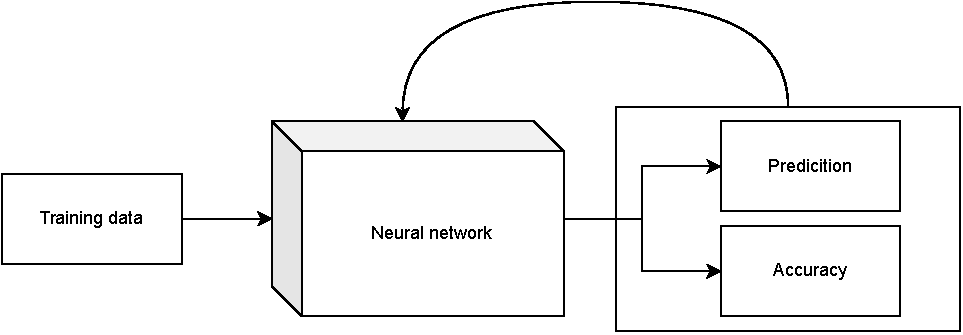
\includegraphics[width=0.8\textwidth]{figures/training.pdf}
	\captionof{figure}[Neural network as blockbox with training data]{Neural network as blockbox with training data}
	\label{fig:training}
\end{minipage}

On the other hand, is the test data. 
In \ref{fig:training} we can see a simplified figure of a neural net as blackbox that uses the test data to make predictions or decisions and compare them to the true values in the test data to evaluate its accuracy and reliability. 
In general, the training data is used to optimize the model and the test data is used to evaluate the model. \cite[p. 32-33]{khan_guide_2018}
%vll. rausmachen
%The data used in the training and test set can be biased in certain directions without the researchers knowing. It could have a higher proportion of males or of a single ethnicity. For example, if a face recognition system is being trained on a data set that mostly consists of white men it will have an easier time identifying white men which will result in a higher success rate.



\vspace{1em}
\begin{minipage}{\linewidth}
	\centering
	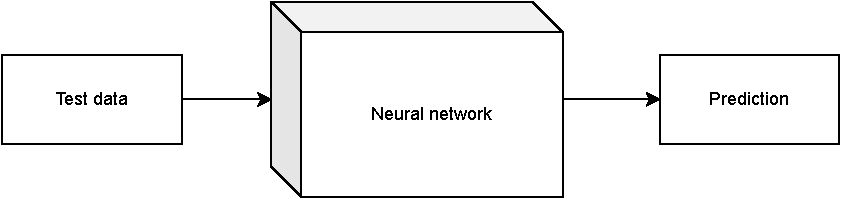
\includegraphics[width=0.8\textwidth]{figures/test.pdf}
	\captionof{figure}[Neural network as blockbox with test data]{Neural network as blockbox with test data}
	\label{fig:test}
\end{minipage}



\chapter{Issues with data}
%TODO Quelle und umschreiben!!
AI bias is an anomaly in the output of machine learning algorithms, due to the prejudiced assumptions made during the algorithm development process or prejudices in the training data.
 
There are many problems concerning the data that can make algorithms unreliable and lead to bias.
One of them is poorly selected data.
The designers of the algorithmic system may decide that certain data is important for the outcome of the algorithm and other data isn't.
This can lead to disadvantages for a certain group of people. \cite[p. 7]{usa}


Another problem is the selection bias.
Selection bias occurs when the set of data inputs to a model is not representative of a population, which can lead to conclusions that favor certain groups over others. \cite[p. 8]{usa}
For example, facial recognition AI algorithms are often trained on data that includes more examples of white people's faces than other races, leading to difficulty in recognizing faces of other races.
In a study by Joy Buolamwini and Timnit Gebru the authors use the Fitzpatrick Skin Type classification system to characterize the gender and skin type distribution of two facial analysis benchmarks, IJB-A and Adience. 
They find that these datasets are overwhelmingly composed of lighter-skinned subjects, and introduce a new facial analysis dataset that is balanced by gender and skin type. 
They evaluate three commercial gender classification systems using their dataset and show that darker-skinned females are the most misclassified group, with error rates of up to 34.7\%. 
The maximum error rate for lighter-skinned males is 0.8\%. 
\cite[p. 1]{buolamwini_gender_2018}

In many databases that algorithms in law enforcement use for identification of suspects people of colour are overly represented and thus matched more frequently. 
This leads to a disproportionate number of both true and false accept. \cite[p. 323-324]{bacchini_race_2019}
This leads to further discrimination when innocent people are stopped, searched or even arrested.
Algorithms working with this kind of data reflect the hidden and historical biases in society that get transferred trough the training data. \cite[p. 8]{usa}



\chapter{How to fight it}
To prevent discrimination in algorithms, there are a number of steps that can be taken. 
One step is to ensure that the training data used to train algorithms is representative of the population it will be used on. 
This can be achieved by using diverse and inclusive data sets, or by using techniques such as data augmentation to make the training data more representative.
Data augmentation is a technique used to increase the amount of training data by adding modified copies of existing data or newly created synthetic data.
The aim of this technique is to reduce overfitting and promote better generalization when training machine learning models. \cite[p. 2]{nanni2022feature}
In the following Figure \ref{fig:augmentation} an example of a image data augmentation on an existing image of a person can be seen. 
This image gets modified in different ways to add more data.

\vspace{1em}
\begin{minipage}{\linewidth}
	\centering
	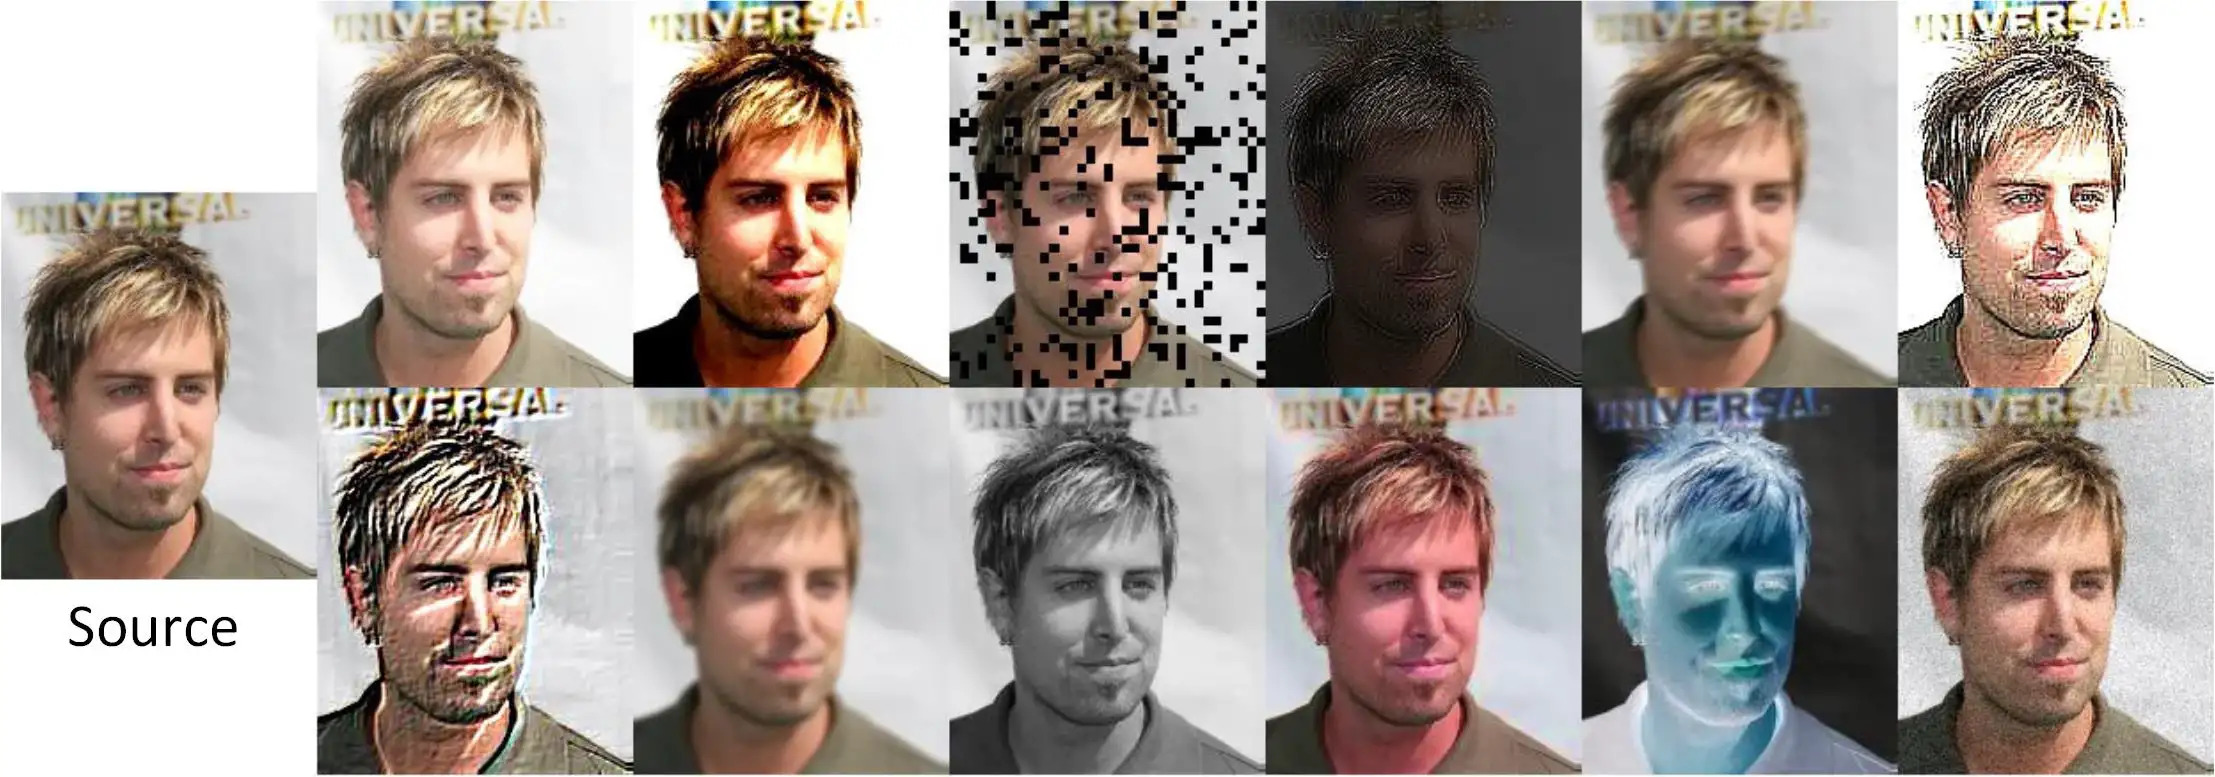
\includegraphics[width=0.8\textwidth]{figures/augmentation2.jpg}
	\captionof{figure}[Example data augmentation]{Example data augmentation \cite{singh_face_2020}}
	\label{fig:augmentation}
\end{minipage}



%\vspace{1em}
%\begin{minipage}{\linewidth}
%	\centering
%	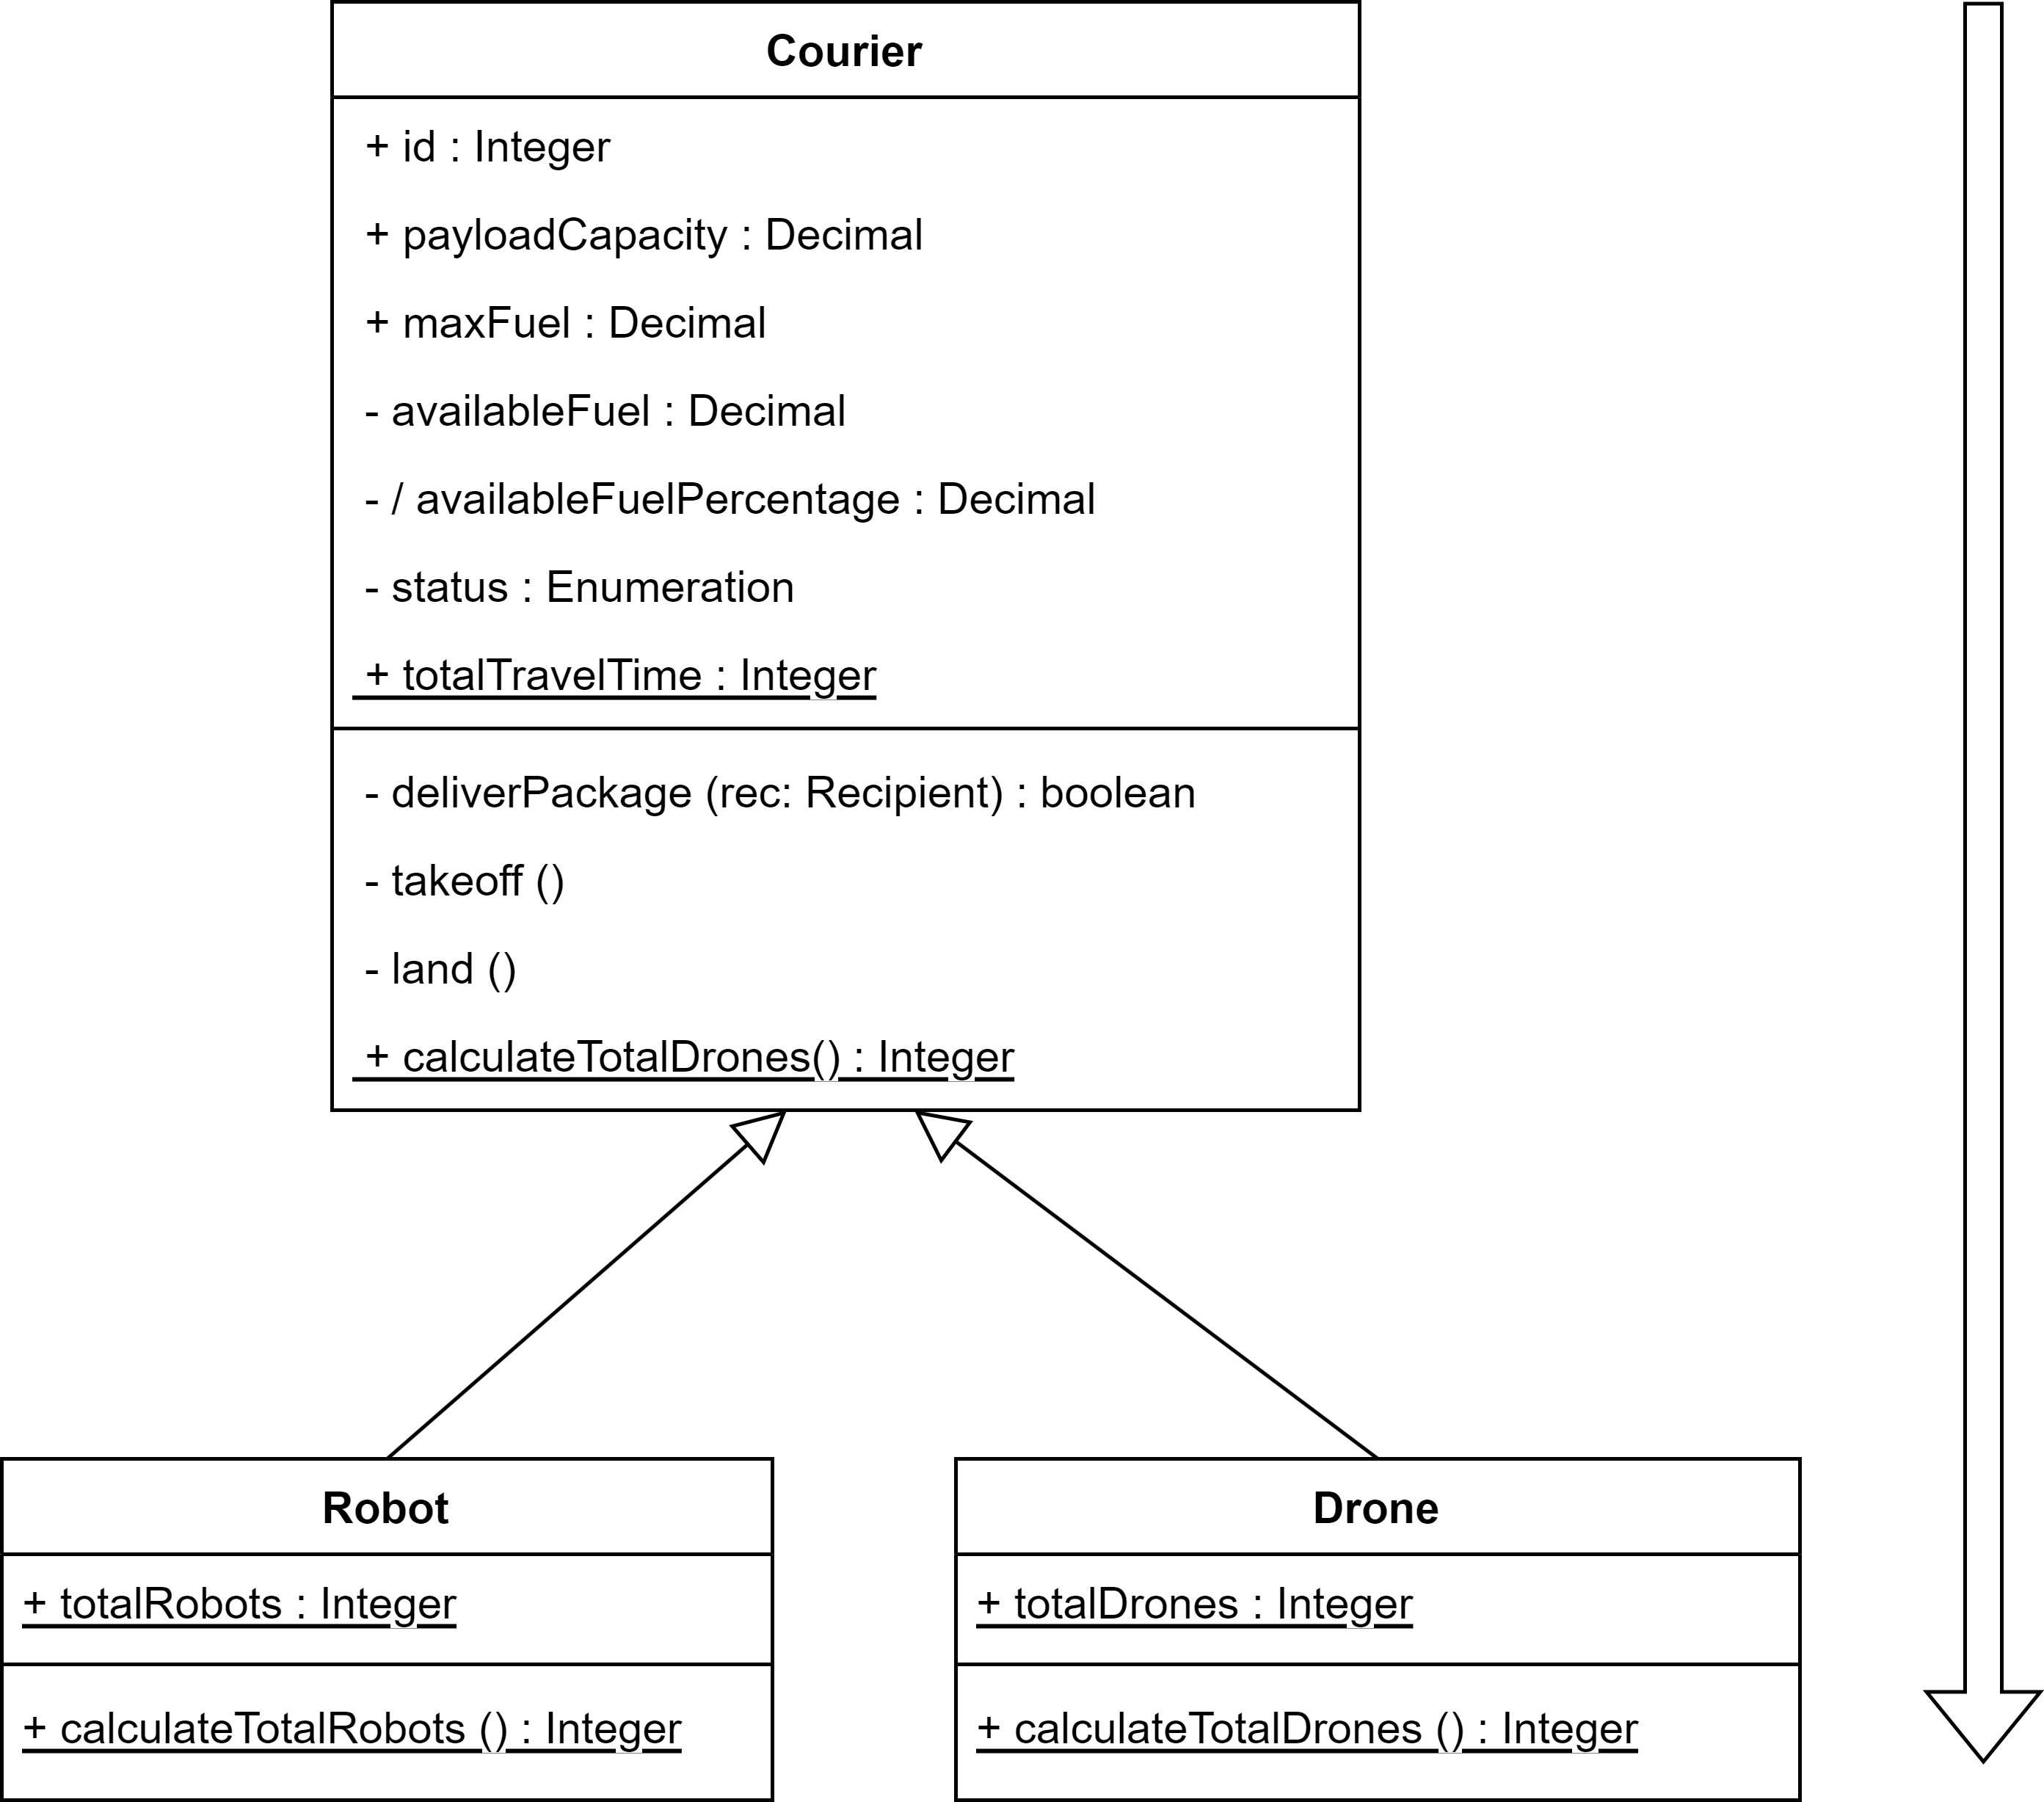
\includegraphics[width=0.7\textwidth]{figures/inheritance/specialization.jpg}
%	\captionof{figure}[Example specialization]{Example of specialization}
%	\label{fig:specialization}
%\end{minipage}





\backmatter
%\listoftodos %remove if no longer needed


% ACHTUNG: ursprüngl: alpha, aber das erzeugt keine Links
%\bibliographystyle{wmaainf}
%\bibliographystyle{alpha}
%\bibliography{refs}
\printbibliography

\clearpage %\cleardoublepage

%-----------------------------------------------------------------------------------------------------------------

%% remove if not needed
%\appendix
%%\pagenumbering{Alph}
%\chapter{Supplemental Information}\label{app:supplemental-information}
%Hier könnte Ihr Anhang stehen!


%-----------------------------------------------------------------------------------------------------------------


\end{document}